\documentclass[11pt]{article}
\usepackage{geometry,tabularx,booktabs,float,natbib}                % See geometry.pdf to learn the layout options. There are lots.
\geometry{letterpaper}                   % ... or a4paper or a5paper or ... 
%\geometry{landscape}                % Activate for for rotated page geometry
%\usepackage[parfill]{parskip}    % Activate to begin paragraphs with an empty line rather than an indent
\usepackage{graphicx}
\usepackage{amssymb}
\usepackage{epstopdf}
\DeclareGraphicsRule{.tif}{png}{.png}{`convert #1 `dirname #1`/`basename #1 .tif`.png}
\newcommand{\myreferences}{references}

\title{Challenges for Head-Mounted Displays}
\author{Juan S. Carrillo}
%\date{}                                           % Activate to display a given date or no date

\begin{document}
\maketitle
\section{Introduction}
Wearables are becoming more and more popular every day. The forms of wearable devices are extremely varied. There are wearables for virtually any part of the body: there are headsets, goggles, glasses, helmets, shirts, vests, bodysuits, armbands, watches, socks, and shoes \cite{VandricoList}. Several years ago it was believed that head-mounted displays (HMD) were going to become the prevalent form in the wearables market \cite{ultimateWearable}. Now there are a large variety of wearables, often smartwatches and smartbands, that are holding their own in the marketplace. This paper argues that currently HMDs face significant challenges that prevent them from becoming as adopted as widely as it was initially predicted.

\section{Background}

Before any further discussion, it is important to note that this paper focuses solely on HMD wearables that are meant to be worn in public. Some HMDs have their own niche in industry and gaming, such as the AirScouter or Oculus. These HMDs are different because of their context and specialization. Wearables that are worn in industry or in private don't face the scrutiny of the general public. Also, highly specialized wearables are targeted to people who want their specific functionality, as in the case of gamers who want to enhance their game playing experience with the Oculus Rift. Since this paper focuses on the widespread assimilation of HMDs, we will not consider these cases.

We will first analyze the background of HMDs and why they were considered by many to be the leading contender for the most popular wearable form. First, we must define what a wearable is. Wearables, broadly, are ``body-worn devices, such as clothing and accessories, which integrate computational capabilities to provide specific features to users"\cite{WearableHumanView}. However, this definition does not include smartphones as they are not body worn devices. In 2001, Starner provided a list of goals for what wearables should be \cite{starnerChallenges1}:
\begin{enumerate}
    \item Persist and provide constant access to information services
    \item Sense and model context
    \item Adapt interaction modalities based on the user's context
    \item Augment and mediate interactions with the user's environment 
\end{enumerate}

In order to \textit{persist and provide constant access to information services}, a wearable must be portable, capable of continuous use, and easily accessible. Starner also added that the device must be physically unobtrusive. A wearable must then be comfortable and discreet. This goal takes into account the dual nature of the wearable both as a computational device and a wearable accessory. Like a watch or a pair of glasses, a wearable must be immediately accessible yet entirely comfortable so that the user is not aware of the device until they need it.  This means that the device will most likely need to be small, lightweight, or otherwise invisible. The wearable can have the form of a familiar accessory such as a pair of glasses, a bracelet or even an article of clothing. The wearable should also be able to discretely interrupt the user in order to give notifications or interact with the user when necessary.

A device that can \textit{sense and model context} is aware of the user's environment and what a user is doing at any given time. The wearable should also be able to tell the user of the wearable's status as well as the user's status. This means that the wearable could make decisions based on the user's context. If a device can detect the user's context, it should be able to \textit{adapt its interaction modalities based on the user's context}. This means that the device can determine what form of interaction with the user is more appropriate given the user's context. The wearable should be versatile enough to discretely inform the user of a status during times such as where the user is in a meeting and be able to interact more directly when the user during times when the user is available and interactions with the wearable are suitable. In other words, the wearable should know the most appropriate way of interacting with the user at any given time.

Finally, a wearable \textit{augments and mediates interactions with the user's environment} by providing information that is relevant to the user based on their location. Whereas the previous two goals focused on the situational context of the user, this goal focuses on how the wearable environmental context. The wearable could filter its notifications based on location and provide additional information based on what the user's current activities. If the user wishes to find a place to eat, the wearable should provide relevant information about local food establishments near the user's location. 

Ten years ago HMDs seemed to be the most obvious form that would satisfy all of these goals. Glasses or any device that could be worn on the user's head would have to be, by necessity, portable and lightweight. Since people detect our surroundings primarily through sight, an HMD with a camera would be able to see everything a user saw and detect the user's context in a similar way. The leading popular head-mounted wearables typically opt to place the display in front of the eyes so as provide information that is instantly available to the user. At the time, HMDs seemed, in theory, to be the ideal wearable paradigm. However, initially HMDs were greatly hindered by technological limitations, which resulted in HMDs that were energy inefficient, bulky, and unwieldy \cite{fromCyborgsToGG}. Early adopters of HMDs admitted that the devices elicited uncomfortable responses from others. Mann, an early adopter of HMDs, pictured in Figure~\ref{fig:Mann}, admitted that at first he did not wear his wearables often, as the devices were both physically and socially awkward \cite{smartClothingShift}.  As a result of the technological limitations, it was difficult for HMDs to become widely accepted.  
% JD: Separate your citations with spaces (I fixed two in the above paragraph).

the leading/most popular head-mounted wearables typically opting to place the display in front of the eyes
% JD: Uh, dangling paragraph/phrase above?

\begin{figure}[H] %  figure placement: here, top, bottom, or page
   \centering
   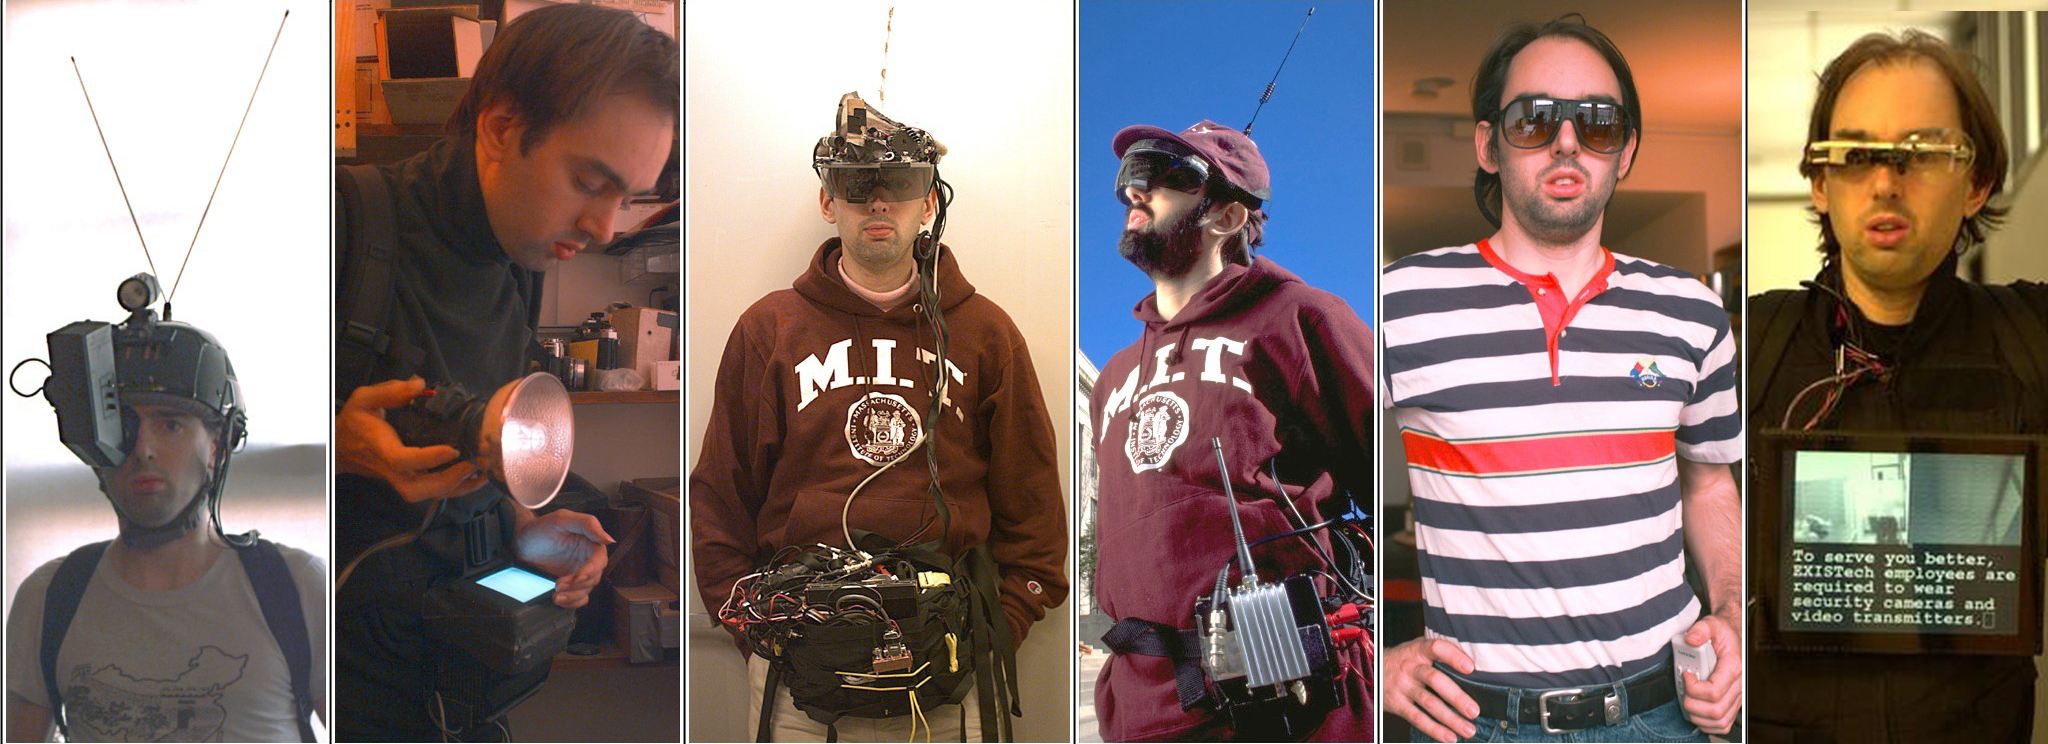
\includegraphics[width=5in]{Wearcompevolution2.jpg}       
   \caption{Prof. Steve Mann with his HMD devices over the years \cite{wearablesOverTime}}
   \label{fig:Mann}
\end{figure} 

In recent years, wearables with head-mounted displays have gotten sleeker, have improved graphics, and are more versatile. An example of this recent trend is Google Glass, which, according to users, is extremely light and comfortable. However, wearables that make use of head-mounted displays still face significant challenges that prevent them from becoming widely adopted. The overall design of HMDs has stayed the same; there is always some kind of screen or display in the users' face. While the design allows for immediate access to information, it also has some unintended social consequences for the user. Another issue that HMD wearables face is the input method for the user, which is severely limited. Finally, another challenge to the widespread adoption of HMDs and to wearables in general is the advent of the smartphone. It is worth noting too that the smartphone fulfills all the criteria for the ideal wearable, except that the phone is not technically a wearable. We will examine these issues more thoroughly in the rest of this paper.
\section{Methods}

One of the main challenges that HMD wearables face as a result of their form is a lack of social acceptance. There are some drawbacks to having a device that is always in front of the user's face. Other people who interact with the user will always see the wearable. Right away, a potential user must consider if they are satisfied with the aesthetic appeal of the wearable. If the user perceives that their image will change in a negative way as a result of using the wearable, they will be deterred from using it \cite{WearableHumanView}. If the user is comfortable with the aesthetic quality of the wearable the user still faces challenges during a face-to-face conversation. During a conversation, most of the time each person will be focused on the other person. Even if the device is cleverly designed so that the device not constantly in the field of vision of the user, as is the case with Google Glass, the device will still be visible to other people. This means that the user's experience with the wearable will depend on other people's attitudes towards the device. In general, most people have not come to accept HMDs in a social context \cite{negativeGlassReactions}. One of the complaints is that wearables hinder conversations between a user and another person \cite{wearableFaceToFace}. A nonuser might perceive that the user has reduced eye contact with the nonuser when the user's wearable is on. Although it could be argued that a wearable user could simply switch off the wearable when they are about to have a conversation with someone, it would negate the principle of a wearable as a device that persists and is always available. Other devices such as a smartwatch or a smartphone, which also give notifications to the user, would not face the same challenge because the nonuser could perceive that the user is still engaged in a conversation if the user does not look at the smartwatch screen or pull out their phone. However, an HMD is always in front of the user's eye, and nonusers would wonder if the user is being distracted by the notification or whether they are still fully engaged in the conversation. Since people greatly value the opinion of their friends and family, potential users could be deterred from using HMD wearables if they feel that it will hinder interacting with those close to them \cite{WearableHumanView}. 

HMDs with recording capabilities also raise concerns about the privacy of nonusers. Google Glass users have reported being treated with hostility or being the subject of criticism as a result of using Glass \cite{fromCyborgsToGG,negativeGlassReactions}.
% JD: Note that you can list multiple cites by separating IDs with commas.
This is explained by the lack of control bystanders have about being recorded by Google Glass users. Whereas ``people make a personal decision[s] to check their smartphone or log in and check their social media accounts, ... Google Glass is out of their control," and so HMDs are understandably uncomfortable for nonusers. While some Glass supporters have claimed that recording people with smartphones is just as discrete as Google Glass because of the ubiquitousness of smartphones, the act of holding up a phone to capture video is much more indicative than recording with Glass. Furthermore, while phones can be put away, wearables are not meant to be put away. The user of a wearable can more easily justify having a recording device constantly out since the wearable is meant to be worn at a ll times, while smartphone users have less of a reason to have their phones out in the open. While the attitudes towards Glass and other HMDs with recording capabilities can change over time despite initial negative reception\cite{changingAttitudes} as of this moment HMDs users face issues with social acceptance as a result of wearing wearables which are perceived as invading people's privacy.

Input is also a serious issue for HMDs wearables. Some simple devices such as Epiphany Eyewear use a single button control. Previously, common ways of interacting with HMDs included an accompanying device such as a controller or a one-handed keyboard \cite{inputForHDMs}. More sophisticated and recent user interfaces allow users to interact with the wearables using a  touch pad, voice, or their phone \cite{inputForHDMs,glassHelp,userInteractionMultipleDisplays}. The issue with additional, third parties devices such as a smartphone as a user interface is that it prevents the HMDs from becoming a standalone devices. Users may be deterred from buying an expensive device that is ultimately dependent on their smartphones in order to function. Some wearables, including Glass, try to appeal to users by allowing them to access information without having to take out their smartphones. These wearables must have another interface independent of the phone. The limited size of the wearable forces HMDs to use small touchpads or use voice commands. The touchpad is incredibly limited because it's so small. It doesn't allow for great flexibility to do complicated tasks. Voice recognition is also limited. Voice recognition software has difficulties understanding what users are saying because voice recognition is difficult and depends on a variety of factors, such as dialects, accents, semantics, and ambient noise\cite{voiceRecognitionTroubles}. Even if the technology was perfected, voice recognition is still limited because it's not always an appropriate or convenient use of input. Speaking to a device is awkward in public spaces, and it creates issues of privacy in cases such as when a user wants to send a private text message.

The widespread assimilation of smartphones is also a large barrier to the adoption of HMDs and wearables in general. When we defined the ideal wearable, we described a device that was always on, always accessible, portable, provided information relevant to the user's context, and could be change the way it interacted with the user. For the most part, smartphones satisfy the criterion of the ideal wearable\cite{fromCyborgsToGG}. A smartphone is portable, instantly accessible, and provides the user with access to information using the internet. Smartphones have large, touch screen interfaces that are far easier to use than the smaller screens of a lot of wearables. Since smartphones don't have to be worn on the user's body, they are less socially intrusive and don't face issues of wearability that wearables have to deal with. In summary, users might have a harder time adopting expensive and unfamiliar hardware that doesn't provide additional functionality when a smartphone can already do most of the things that wearables can do.  

\section{Discussion}

We have now considered some of the major challenges that HMD wearables face that prevent them from being widely adopted by the general populace. We will now consider how these challenges translate in terms of the usability of HMDs.  Ultimately, the perceived usability of a device plays a crucial role in whether or not users will want to adopt the wearable\cite{WearableHumanView}\cite{UserAcceptance}\cite{WhyUsersDont}\cite{hmdOlderAdults}(and many others!). We will briefly elaborate about each of these criteria: \textit{learnability} is concerned on how long it takes and how easy it is for users to adopt an interface; \textit{efficiency} is how long it takes a user to complete a typical task; \textit{errors} measure the rate of errors by users; \textit{memorability} is the retention of how to use the interface over time by users; \textit{satisfaction} is the subjective fulfillment or enjoyment that users derive from using an interface. 

In terms of usability, HMDs are deficient in the satisfaction and errors metric. Users are hesitant to adopt a new product if the product is not socially acceptable. HMDs are perceived are often perceived as hindering direct, interpersonal conversation. HDMs users, in particular Google Glass users, risk confrontation with bystanders who feel that their own personal privacy is being invaded by the user's device. There has even been a derisive term coined for Glass users:``Glassholes"\cite{negativeGlassReactions}. If the device is not socially acceptable and a target of criticism, the user's overall enjoyment diminishes. HMDs are especially visible as they are worn on the users head, and as a wearable are meant to be worn all the time. If the user has to constantly remove his or her own wearable in order to avoid criticism or looks of disapproval, then the technology that was meant to enhance their personal experience will actually become an inconvenience. 

Any HMD that has a limited user interface can also frustrate users. An interface that is based on voice commands can be especially frustrating become voice recognition software is still error prone. Voice commands are not appropriate for instance when the user desires privacy. In comparison to multi-touch interfaces or point-and-click interfaces, voice commands are much more difficult, error prone, and less versatile. While the novelty of having a computer that voice commands is exciting, users will ultimately use an interface that is efficient and less error prone. 

Finally, HMDs have to compete with smartphones. Smartphones can for the most part do everything a wearable can do, and more. It is more portable than a laptop and more usable than a wearable. It is general purpose, relatively cheap (compared to Google Glass), and socially acceptable. It will be difficult for users to want to adopt a wearable with so many drawbacks when there is already a technology that can do everything a wearable can do.
% JD: Ah, just when you were warming up!  The sections prior to Discussion are very informative
%     and decently written, but what you have done *here* is the meat and potatoes of the paper,
%     and it is a pity that it has stopped short.  The comparison with smart phones, especially
%     can be quite rich---in particular, interaction styles would be good to examine.  Today's
%     smartphones are capable of virtually all interaction styles, but not today's wearables
%     (much less HMDs).  I think it would be interesting to see whether this situation is
%     temporary (e.g., once upon a time smartphones were just as limited as HMDs in terms of
%     interaction style), or intrinsic/permanent (i.e., HMD size and display limitations might
%     forever preclude some styles).

\section{Conclusion}

There are significant challenges that inhibit the widespread adoption of head-mounted wearables. These challenges are inherent to the wearable's form. In order for users to be willing to adopt wearables to the same degree as laptops or smartphones, designers must come up with innovative approaches to deal with these issues. As of right now, the author firmly believes that wearables will not be widely adopted in the near future.

\bibliographystyle{unsrt}
\bibliography{\myreferences}

\end{document}  